% Preprint — Sigma Transfer and Fiber Overlap. Author: Derek Blair <derekjblair@gmail.com>
% Source data: ~/workspace/math-unsolved/ROUND275_DOSSIER.md (2026-10-10),
%              ~/workspace/math-unsolved/ROUND298_DOSSIER.md (2026-10-10),
%              ~/workspace/math-unsolved/ROUND310_DOSSIER.md (2026-10-11),
%              ~/workspace/math-unsolved/ROUND277_DOSSIER.md (2026-10-10),
%              ~/workspace/math-unsolved/ROUND294_DOSSIER.md (2026-10-10);
%              Lean modules ~/workspace/math-unsolved/lean/Mathproofs/SigmaTrans.lean
%              and ~/workspace/math-unsolved/lean/Mathproofs/FiberOverlap.lean.
% All figures native TikZ/pgfplots; all tables booktabs.
\documentclass[11pt,a4paper]{article}
\usepackage{amsmath,amssymb,amsthm}
\usepackage{tikz}
\usetikzlibrary{positioning,shapes,arrows.meta}
\usepackage{pgfplots}
\pgfplotsset{compat=1.18}
\usepackage{booktabs}
\usepackage{geometry}
\geometry{margin=2.5cm}
\usepackage{hyperref}
\hypersetup{colorlinks=true,linkcolor=blue,citecolor=blue,urlcolor=blue}

\newtheorem{theorem}{Theorem}
\newtheorem{proposition}{Proposition}
\newtheorem{lemma}{Lemma}
\newtheorem{corollary}{Corollary}
\theoremstyle{definition}
\newtheorem{assumption}{Assumption}

\title{Sigma Transfer and Fiber Overlap:\\
  Pareto Transitions of the March-Graph Spectrum and the Sidon
  Fiber-Overlap Bound}
\author{Derek Blair \\ \texttt{derekjblair@gmail.com}}
\date{October 2026}

\begin{document}
\maketitle

%======================================================================
\section{Abstract}
%======================================================================

We study the $\sigma$-spectrum $S(\sigma)$ of the march-graph program:
the set of attainable $(|E|,|S|)$ classes at span $\sigma$ over the
$5{,}872$-shape universe of Sidon $9$-shapes, and its Pareto frontier
$\Pi(\sigma)$. The formalized content, all [PROVED] in Lean, is the
\emph{$\sigma$-transfer} suite (T5, T6, T7$'$, T8$'$) and the
\emph{fiber-overlap} suite. The transfer theorems: Pareto membership is
down-set membership (Theorem~\ref{thm:pareto}, \texttt{mem\_paretoMin\_
iff}); every class's transition status across an adjacent span pair is a
function of per-class down-set queries on the two spectra
(Theorem~\ref{thm:t5}, \texttt{status\_local}: the T5 locality bar, old
spectra only); the axioms A1--A3 impose no relation between consecutive
spectra, witnessed by three explicit abstract models
(Theorem~\ref{thm:t6}, \texttt{no\_forcing\_equality}/
\texttt{\_disjoint}/\texttt{\_sharing}: the T6 abstract-only bar);
reflection duals of Pareto classes are never distinct Pareto classes
(Theorem~\ref{thm:dual}, \texttt{dual\_emin}, \texttt{no\_cotransition},
\texttt{A3\_holds}). The fiber theorems: distinct pair-sum fibers of a
Sidon set overlap in at most one point
(Theorem~\ref{thm:fiberoverlap}, \texttt{fiber\_overlap},
\texttt{fiber\_overlap\_identity}, \texttt{autocorr\_le\_one}), and
top-interval sparsity holds conditionally on the [PROVED*] T1/T2 floors
(Theorem~\ref{thm:sparsity}, \texttt{top\_interval\_sparsity}).
We also record, honestly, that Q-20's claimed sharp Pareto floor
$|E|=0\implies|S|\ge7$ is refuted by an exact six-hole witness
(Proposition~\ref{prop:q20}, [COMPUTED]).

%======================================================================
\section{Introduction}
%======================================================================

A Sidon set $A$ (a $B_2$ set) has all pair sums $a+b$ ($a,b\in A$)
essentially distinct. The march-graph program studies Sidon $9$-shapes
$A=\{0=a_0<\dots<a_8=\sigma\}$ of span $\sigma\le183$ through their
\emph{pair-sum shadow} $(D,H,W)$ and the $(E,S)$ hole counts
(R264/R270/R273, cited as given). For each span $\sigma$ the
\emph{$\sigma$-spectrum} $S(\sigma)$ is the set of attainable
$(|E|,|S|)$ classes over the $5{,}872$-shape universe, and its
$\le$-minimal elements form the \emph{Pareto frontier} $\Pi(\sigma)$
($195$ distinct classes over $294$ instances in the census, supplied
datum). The program's transition analysis (R275) classifies, for each
adjacent pair $\sigma\to\sigma+1$, how Pareto classes persist, demote,
vanish, appear, or promote --- the \emph{transition DAG} further studied
in the companion paper on transition DAGs.

This paper's formalized contribution is the abstract, machine-checked
core of that analysis, kept strictly within what the Lean modules prove:
\begin{enumerate}
\item The down-set characterization of Pareto membership and the T5
  transition-locality law (Theorems~\ref{thm:pareto}--\ref{thm:t5}).
\item The T6 no-forcing theorem: three explicit abstract spectra show
  the floor axioms impose no relation between consecutive spectra
  (Theorem~\ref{thm:t6}).
\item The T7$'$/T8$'$ dual statements for full-normalized-universe
  reflection (Theorem~\ref{thm:dual}).
\item The fiber-overlap identity and bound, and the conditional
  top-interval sparsity law (Theorems~\ref{thm:fiberoverlap},
  \ref{thm:sparsity}).
\end{enumerate}
Every census number in this paper is [COMPUTED] ($\times2$, two
independent paths, exact agreement) and is never re-claimed as a
theorem; every theorem is an abstract Lean-checked statement. The
six-hole witness of Proposition~\ref{prop:q20} is a [COMPUTED]
refutation we keep on the record.

%======================================================================
\section{Methods}
%======================================================================

\subsection{Definitions}

We use the R264/R270/R273 notation (supplied datum). Fix a Sidon
$9$-shape $A=\{0=a_0<\dots<a_8=\sigma\}$ of span $\sigma\le183$.
\begin{itemize}
\item $P$ is the set of $45$ pair sums $a+b$.
\item $D=\bigcup_{s\in P}(s-A)$ is the union of the $45$ \emph{D-fibers}
  $f_s=s-A$.
\item $H=\{s/2:s\in P\text{ even}\}$ and $W=D\cup H$ ($A\subseteq D$).
\item $u=183-\sigma$; $J=[\sigma-183,-1]$.
\item $E=J\setminus D$ and $S=[0,\sigma]\setminus W$; $|G_{t_{\max}}|=
  |E|+|S|$.
\end{itemize}
$S(\sigma)$ is the $\sigma$-spectrum: the set of attainable
$(|E|,|S|)$ classes at span $\sigma$ over the $5{,}872$-shape universe.
$\Pi(\sigma)$ is the Pareto frontier: the $\le$-minimal elements of
$S(\sigma)$. In Lean:
$\mathtt{paretoMin}(S)=S.\mathrm{filter}(\lambda p.\,\forall q\in S,\,
q\le p\to q=p)$ and
$\mathtt{downSet}(S,c)=S.\mathrm{filter}(\cdot\le c)$.

The R275 transition taxonomy (supplied datum) over an adjacent pair
$\sigma\to\sigma+1$ with spectra $S,S'$ assigns each class one of five
statuses (Lean inductive \texttt{Status}):
\texttt{persist}, \texttt{demoted}, \texttt{extinct},
\texttt{fresh}, \texttt{promoted}. In down-set form: persist $\iff$
$c\in S'\land(\mathord\downarrow(c)\setminus\{c\})\cap S'=\varnothing$;
demoted $\iff$ $c\in S'\land(\mathord\downarrow(c)\setminus\{c\})\cap
S'\neq\varnothing$; extinct $\iff$ $c\notin S'$; promoted $\iff$
$a\in S(\sigma)\setminus\Pi(\sigma)$ with blockers
$\Pi(\sigma)\cap\mathord\downarrow(a)\neq\varnothing$; fresh $\iff$
$a\notin S(\sigma)$.

The three floor axioms (Lean \texttt{A1}, \texttt{A2}, \texttt{A3}):
\begin{itemize}
\item A1 (floor): every class of $S$ has $e\ge\mathrm{floor}$,
  $\mathrm{floor}(\sigma)=183-2\sigma$.
\item A2 (reflection-closure): the reflected $e$-value appears at the
  same $s$.
\item A3 (Pareto): $\Pi(S)$ is the $\le$-minimal set (definitional).
\end{itemize}
The T6 forcing models are three explicit abstract spectra with
$m=\max(f(\sigma),f(\sigma+1))$ and identity reflection: the
\emph{equality} model $S=S'=\{(m,0)\}$; the \emph{disjointness} model
$S=\{(m,0)\}$, $S'=\{(m,1)\}$; the \emph{sharing} model
$S=S'=\{(m,1),(m+1,0)\}$ (an antichain).

For the fiber suite: the \emph{fiber} of $A$ at shift $s$ is
$f_s=s-A=\{s-a:a\in A\}$ (Lean
$\mathtt{fiber}(A,s)=A.\mathrm{image}(\lambda a.\,s-a)$). The
\emph{autocorrelation} of $A$ at $t$ is $|A\cap(A+t)|$.
\emph{Top-interval sparsity} is the bound $|D\cap[\sigma+1,183]|\le
\sigma$ for $\sigma\le91$, derived from T2's equality
$|E_{\bar A}|=u-|D_A\cap[\sigma+1,183]|$ and T1's $|E_{\bar A}|\ge
183-2\sigma$ (both [PROVED*], cited with labels intact). Conjecture~F
fragments: F1: $|E|=0\implies|S|\ge2$; F2: $|S|=0\implies|E|\ge2$;
Conjecture~F: $|E|+|S|\ge2$ for all Sidon $9$-shapes.

\subsection{Formalization note}
\label{sec:formalization}

The machine-checked content lives in the repository
\texttt{derekblair/math-proofs}, Lean~4.34.1 with Mathlib pinned at
commit \texttt{d13f23b}. Verification config: full-library
\texttt{lake build} on the bakkie fleet machine (2026-10-11, 11:12~PDT):
``Build completed successfully (17936 jobs)'' --- exit~$0$, $0$ errors,
$0$ \texttt{sorry}s, $0$ \texttt{admit}s in the log. The R310 label move
took both modules from [PROVED*] to [PROVED] (charter rule~4), with
\texttt{SigmaTrans} (Q-22) and \texttt{FiberOverlap} (Q-23) among the
$8$ queue modules built. Modules are md5-identical
local~$\leftrightarrow$~bakkie (\texttt{SigmaTrans.lean}
\texttt{ab2398b4$\dots$}; \texttt{FiberOverlap.lean}
\texttt{67b2a9a5$\dots$}), each registered exactly once per side. Axiom
audits: \texttt{SigmaTrans} standard-only
\texttt{[propext, Classical.choice, Quot.sound]};
\texttt{autocorr\_le\_one}, \texttt{fiber\_overlap\_identity},
\texttt{fiber\_overlap}: \texttt{[propext, Classical.choice,
Quot.sound]}; \texttt{f\_iff\_f1\_f2}, \texttt{top\_interval\_sparsity}:
\texttt{[propext, Quot.sound]}. Each module's header points at this
paper's slug
\texttt{papers/sigma-transfer-fiber-overlap-October-11-2026/}; this
paper points back at the modules and the exact theorem names of
Table~\ref{tab:formalization}.

\begin{table}[t]
  \centering
  \caption{Formalized theorems, all [PROVED]. Module paths are
    repo-relative.}
  \label{tab:formalization}
  \begin{tabular}{lll}
    \toprule
    Lean theorem & content & axioms \\
    \midrule
    \multicolumn{3}{l}{\texttt{Mathproofs/SigmaTrans.lean}} \\
    \ \ \texttt{mem\_paretoMin\_iff} & Pareto $\iff$ down-set singleton
      & standard \\
    \ \ \texttt{status\_local} & T5 transition locality & standard \\
    \ \ \texttt{dag\_deterministic} & statuses exhaustive/total & standard \\
    \ \ \texttt{demoter\_exists} & finite descent to Pareto & standard \\
    \ \ \texttt{dual\_emin} & T7$'$ dual $e$-min & standard \\
    \ \ \texttt{no\_cotransition} & T8$'$ no distinct co-Pareto dual
      & standard \\
    \ \ \texttt{A3\_holds} & Pareto axiom holds & standard \\
    \ \ \texttt{no\_forcing\_equality} & T6 equality model & standard \\
    \ \ \texttt{no\_forcing\_disjoint} & T6 disjoint model & standard \\
    \ \ \texttt{no\_forcing\_sharing} & T6 sharing model & standard \\
    \multicolumn{3}{l}{\texttt{Mathproofs/FiberOverlap.lean}} \\
    \ \ \texttt{autocorr\_le\_one} & autocorrelation $\le1$ & standard \\
    \ \ \texttt{fiber\_overlap\_identity} & overlap $=$ autocorrelation
      & standard \\
    \ \ \texttt{fiber\_overlap} & fiber-overlap bound & standard \\
    \ \ \texttt{f\_iff\_f1\_f2} & F $\iff$ F1$\land$F2 (pure logic)
      & \texttt{[propext, Quot.sound]} \\
    \ \ \texttt{top\_interval\_sparsity} & sparsity (conditional)
      & \texttt{[propext, Quot.sound]} \\
    \bottomrule
  \end{tabular}
\end{table}

The scope bar (Q-22, quoted scoped SURVIVES, 2026-10-10~21:31~PDT; Q-23,
quoted SURVIVES, 2026-10-10~21:25~PDT) is part of the claim:
T5 is \emph{old-spectrum queries} only --- each class's status is a
function of per-class down-set queries on the two spectra; the census
data itself stays [COMPUTED]. T6 is \emph{abstract A1--A3 only} --- the
three models are Lean-checked existence statements over abstract
finsets. T2$'$/T7$'$/T8$'$ are \emph{full-normalized-universe} results
with witness-level reflection (abstract reflection endomap with
$s$-preservation); the per-shape T2$'$ content
(\texttt{reflection\_per\_shape}, needing the $(S,E)$ evaluator
formalized) is DEFERRED, documented in the module header, and not
claimed here. The $103$-pair transition census, the $558$-case T5
down-set audit, the T6 model audits, the T2$'$/T7$'$/T8$'$ scripted
audits, and the $5{,}813{,}280$-pair fiber audit stay [COMPUTED]$\times2$.

%======================================================================
\section{Results}
%======================================================================

\begin{theorem}[Pareto membership; PROVED]
  \label{thm:pareto}
  For $S$ a finset of $\mathbb{N}\times\mathbb{N}$ and $c$ a class,
  \begin{equation}
    \label{eq:pareto}
    c\in\mathtt{paretoMin}(S)\;\Longleftrightarrow\;
    c\in S\ \land\ \mathtt{downSet}(S,c)=\{c\}.
  \end{equation}
\end{theorem}

\begin{theorem}[T5 transition locality; PROVED]
  \label{thm:t5}
  The transition status of a class $c$ across adjacent spectra $S,S'$
  is a function of per-class down-set queries on the two spectra:
  \texttt{transStatus} is defined by cases on
  $c\in S\land\mathtt{downSet}(S,c)=\{c\}$ and the same predicate on
  $S'$, and \texttt{dag\_deterministic} shows the five statuses are
  exhaustive and total over $\Pi(S)\cup\Pi(S')$. Moreover
  (\texttt{demoter\_exists}), every non-Pareto class descends to a
  Pareto class: $c\in S$, $c\notin\mathtt{paretoMin}(S)$ implies
  $\exists q\in\mathtt{paretoMin}(S)$ with $q\le c$, $q\neq c$.
\end{theorem}

Theorem~\ref{thm:t5} is the entire content of T5 that we claim: the
status function is \emph{local} to the two spectra's down-set data.
Nothing about the census's actual statuses is proved in Lean; the
$558$-record audit (below) is a supplied [COMPUTED] datum. The
orientation of demote edges was additionally audited on the census
($24$ demote edges, $0$ orientation errors, supplied datum).

\begin{figure}[t]
  \centering
  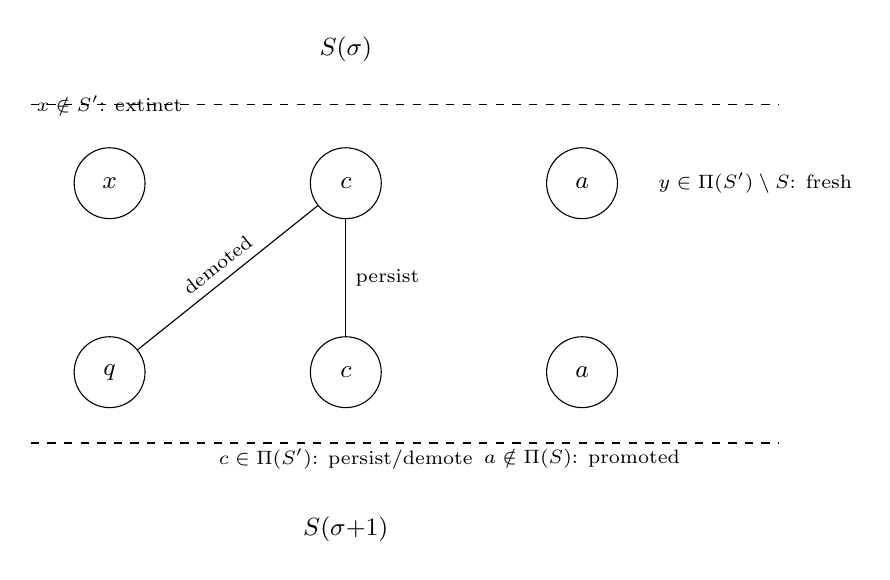
\begin{tikzpicture}[
      node distance=1.6cm,
      cls/.style={draw, circle, minimum size=0.9cm, font=\small},
      every edge/.style={draw, -{Stealth[scale=0.8]}},
    ]
    \node[cls] (c) at (0,2.4) {$c$};
    \node[cls] (cp) at (0,0) {$c$};
    \node[cls] (q) at (-3,0) {$q$};
    \node[cls] (a) at (3,2.4) {$a$};
    \node[cls] (ap) at (3,0) {$a$};
    \node[cls] (x) at (-3,2.4) {$x$};
    \draw (c) -- (cp) node[midway,right,font=\scriptsize] {persist};
    \draw (c) -- (q) node[midway,above,font=\scriptsize,sloped] {demoted};
    \node[font=\scriptsize] at (-3,3.4) {$x\notin S'$: extinct};
    \node[font=\scriptsize] at (3,-1.1) {$a\notin\Pi(S)$: promoted};
    \node[font=\scriptsize] at (0,-1.1) {$c\in\Pi(S')$: persist/demote};
    \node[font=\scriptsize] at (5.2,2.4) {$y\in\Pi(S')\setminus S$: fresh};
    \node[draw=none,font=\small] at (0,4.1) {$S(\sigma)$};
    \node[draw=none,font=\small] at (0,-2) {$S(\sigma{+}1)$};
    \draw[dashed] (-4,3.4) -- (5.5,3.4);
    \draw[dashed] (-4,-0.9) -- (5.5,-0.9);
  \end{tikzpicture}
  \caption{The T5 transition taxonomy (Theorem~\ref{thm:t5}): a class's
    status across $S(\sigma)\to S(\sigma+1)$ is read off from per-class
    down-set queries on the two spectra. Arrows show persist
    ($c\in\Pi$ both sides) and demoted ($c$ lands on a dominating
    $q$); extinct, fresh, and promoted complete the five statuses.}
  \label{fig:taxonomy}
\end{figure}

\begin{theorem}[T6 no-forcing; PROVED]
  \label{thm:t6}
  The axioms A1--A3 impose no relation between consecutive spectra.
  There exist abstract finsets satisfying A1--A3 at both spans with
  (i)~identical Pareto minima (\texttt{no\_forcing\_equality},
  $\{(m,0)\}$ both sides), (ii)~disjoint Pareto minima
  (\texttt{no\_forcing\_disjoint}, $\{(m,0)\}$ vs $\{(m,1)\}$), and
  (iii)~an identical two-class antichain
  (\texttt{no\_forcing\_sharing}, $\{(m,1),(m+1,0)\}$ both sides, card
  $2$), where $m=\max(f(\sigma),f(\sigma+1))$ and the reflection is the
  identity endomap.
\end{theorem}

The claim is deliberately \emph{existential and abstract}: the models
are Lean-checked witnesses that the axioms do not force
persist/demote/extinct/fresh/promote patterns. The census fact that
$103/103$ consecutive frontier sets are distinct is contingent and
[COMPUTED], not a class-level law and not a theorem (supplied datum,
R275 dossier). In particular, ``nowhere $\sigma$-monotone is a
frontier-set-level census fact, not a class-level law and not a
theorem.''

\begin{theorem}[T7$'$/T8$'$ dual statements; PROVED]
  \label{thm:dual}
  Let $r$ be a reflection endomap on the class universe with
  $s$-preservation ($\forall p,\,(rp).2=p.2$). Then
  (\texttt{dual\_emin}): if $p\in\mathtt{paretoMin}(S)$ and
  $rp\in S$, then $p.1\le(rp).1$; and (\texttt{no\_cotransition}): if
  further $rp\in\mathtt{paretoMin}(S)$, then $rp=p$ --- the dual of a
  Pareto class is never a distinct Pareto class. Moreover
  (\texttt{A3\_holds}) the Pareto axiom holds for all $S$.
\end{theorem}

These are full-normalized-universe statements with witness-level
reflection (Q-22 scoped bar): $\sigma$-internality is captured by $r$
being an endomap on the class universe. The census's T7$'$/T8$'$ scripted
audits are [COMPUTED], not formalized; R273's original T2
census-universe conclusion is FALSE ([COMPUTED] decisive: $51/294$
Pareto instances have a witness whose reflection dual $(e',s)$ satisfies
$e'<e$; $3937/5872$ shapes' dual classes are absent from their span's
census spectrum --- the census spectrum is not reflection-closed,
affecting $83\%$ of Pareto instances; supplied datum, R275 dossier).

\begin{table}[t]
  \centering
  \caption{Transition census (supplied [COMPUTED]$\times2$ datum, R275
    dossier; two independent paths, exact agreement). None of these
    numbers is a theorem.}
  \label{tab:census}
  \begin{tabular}{lr}
    \toprule
    quantity & value \\
    \midrule
    shapes in universe & $5{,}872$ \\
    adjacent-pair transition records & $103$ \\
    distinct Pareto classes & $195$ \\
    Pareto-class instances & $294$ \\
    class-transition records & $558$ \\
    dominance-logic events ($20$ demoted $+$ $13$ promoted) & $33$ ($5.8\%$) \\
    persist events (over $13$ pairs; max share $2$ at $86{>}87$) & $14$ \\
    merges / splits & $3$ / $4$ \\
    demote edges (orientation-audited) & $24$ \\
    extinct $+$ fresh (sampling churn) & $259+266$ \\
    vanish total $=$ appear total & $279$ \\
    \bottomrule
  \end{tabular}
\end{table}

\begin{figure}[t]
  \centering
  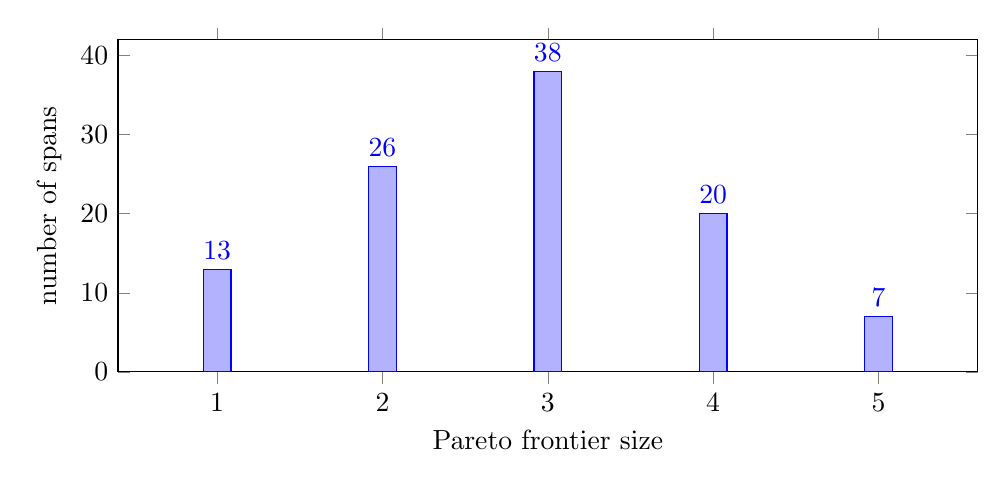
\begin{tikzpicture}
    \begin{axis}[
      ybar, bar width=10pt,
      width=12.5cm, height=5.8cm,
      ymin=0, ymax=42,
      symbolic x coords={1,2,3,4,5},
      xtick=data,
      xlabel={Pareto frontier size},
      ylabel={number of spans},
      nodes near coords,
      enlarge x limits=0.15,
    ]
    \addplot coordinates {(1,13) (2,26) (3,38) (4,20) (5,7)};
    \end{axis}
  \end{tikzpicture}
  \caption{Distribution of Pareto frontier sizes $|\Pi(\sigma)|$ across
    the $103$ adjacent-pair records (supplied [COMPUTED] datum, R275
    dossier).}
  \label{fig:frontierbars}
\end{figure}

\begin{theorem}[Fiber-overlap; PROVED]
  \label{thm:fiberoverlap}
  Let $A$ be a Sidon set (Lean \texttt{IsSidon}: $a+b=c+d$ implies
  $\{a,b\}=\{c,d\}$ as multisets). Then:
  \begin{enumerate}
  \item (\texttt{autocorr\_le\_one}) for $t\neq0$,
    \begin{equation}
      \label{eq:autocorr}
      |A\cap(A+t)|\le1;
    \end{equation}
  \item (\texttt{fiber\_overlap\_identity}) for all shifts $s,s'$,
    \begin{equation}
      \label{eq:fiberid}
      |(s-A)\cap(s'-A)|=|A\cap(A+(s-s'))|;
    \end{equation}
  \item (\texttt{fiber\_overlap}, the Fiber Overlap Lemma) for
    $s\neq s'$,
    \begin{equation}
      \label{eq:fiberoverlap}
      |(s-A)\cap(s'-A)|\le1.
    \end{equation}
  \end{enumerate}
\end{theorem}

The identity~\eqref{eq:fiberid} is the bridge: fiber overlap
\emph{is} autocorrelation, and autocorrelation is $\le1$ for Sidon sets
because two distinct representations of a shift would give two distinct
pair-sum decompositions. The module additionally proves
\texttt{f\_iff\_f1\_f2} [PROVED, pure logic]: Conjecture~F
($|E|+|S|\ge2$ for all Sidon $9$-shapes) holds iff both F1
($|E|=0\implies|S|\ge2$) and F2 ($|S|=0\implies|E|\ge2$) hold. The
$5{,}813{,}280$-pair fiber audit found $0$ mismatches of the identity,
$0$ violations of the $\le1$ bound, and $0$ cases of autocorrelation
$>1$ (supplied [COMPUTED]$\times2$ datum, R277 dossier).

\begin{theorem}[Top-interval sparsity, conditional; PROVED]
  \label{thm:sparsity}
  For $\sigma\le91$, given $d\le u$ with $u=183-\sigma$,
  $u-d=e$ (T2 equality, hypothesis \texttt{hT2}), and
  $e\ge183-2\sigma$ (T1 $E$-floor, hypothesis \texttt{hT1}),
  \begin{equation}
    \label{eq:sparsity}
    d\le\sigma,
  \end{equation}
  i.e.\ $|D\cap[\sigma+1,183]|\le\sigma$.
\end{theorem}

Theorem~\ref{thm:sparsity} (\texttt{top\_interval\_sparsity}) is
[COMPUTED] on $377$ universe shapes with $\sigma\le91$, $0$ violations
(supplied datum, R277 dossier), and [PROVED] as a Lean conditional. The
condition is essential: T1 and T2 are [PROVED*] (R273), cited here with
labels intact and never used as established fact. The Q-23 review scope
is exactly the three fiber lemmas; the scripted audit and the
$\lceil u/9\rceil$ fiber-budget tightening application are not
formalized.

\begin{proposition}[Q-20 refuted; COMPUTED]
  \label{prop:q20}
  The claim ``$|E(A)|=0\implies|S(A)|\ge7$ for every Sidon $9$-shape''
  is false. The exact witness (fresh code path
  \texttt{r294\_q20\_verify.py}, $9\times9$ pair-sum grid deduped,
  plain set loops; result JSON \texttt{r294\_q20\_verify.json}) is
  \begin{equation}
    \label{eq:sixhole}
    A=\{0,29,43,74,82,83,93,109,169\},\quad\sigma=169,
  \end{equation}
  a valid Sidon $9$-shape ($|P|=45$) with $E=\varnothing$ and
  \begin{equation}
    S=\{5,25,46,141,145,151\},\qquad |S|=6<7,
  \end{equation}
  $|D|=262$, $|H|=27$, $|J|=14\subseteq D$ (supplied datum, R294
  dossier).
\end{proposition}

\begin{figure}[t]
  \centering
  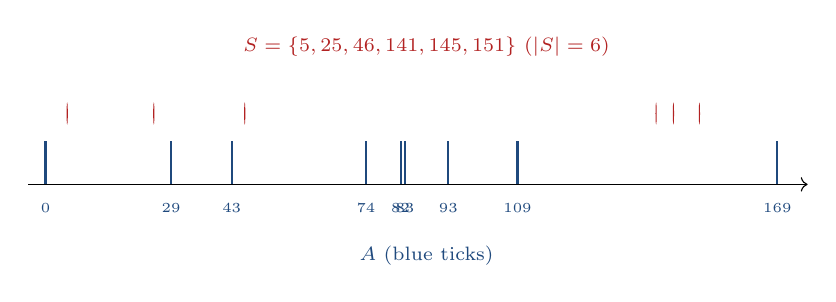
\begin{tikzpicture}[xscale=0.055, yscale=1]
    \definecolor{hole}{RGB}{178,34,34}
    \definecolor{shape}{RGB}{31,73,125}
    \draw[->] (-4,0) -- (176,0);
    \foreach \x in {0,29,43,74,82,83,93,109,169}
      \draw[color=shape,thick] (\x,0) -- (\x,0.55);
    \foreach \x/\lab in {0/0,29/29,43/43,74/74,82/82,83/83,93/93,109/109,169/169}
      \node[color=shape,font=\tiny,anchor=north] at (\x,-0.12) {\lab};
    \foreach \x in {5,25,46,141,145,151}
      \fill[hole] (\x,0.9) circle (4pt);
    \node[hole,font=\scriptsize] at (88,1.75) {$S=\{5,25,46,141,145,151\}$ ($|S|=6$)};
    \node[color=shape,font=\scriptsize] at (88,-0.9) {$A$ (blue ticks)};
  \end{tikzpicture}
  \caption{The six-hole witness of Proposition~\ref{prop:q20}: the Sidon
    $9$-shape~\eqref{eq:sixhole} has $|E|=0$ but only six $S$-holes
    (red), refuting the claimed $|S|\ge7$ floor. Data from
    \texttt{r294\_q20\_verify.json} (supplied datum, R294 dossier).}
  \label{fig:sixhole}
\end{figure}

Consequently Conjecture~F's O1 branch is not closed by this route;
F1/F2 remain [OPEN] (Q-11, Dot-owned, cited as an open dependency).
R270's sweep re-analysis stands: $40$ spans achieve true $|E|=0$
(min $|S|=7$ at $\sigma=158$); $18$ spans true $|S|=0$ (min $|E|=5$ at
$\sigma\in\{116,130\}$) (supplied datum, R277 dossier). We do not
claim the refuted floor anywhere in this paper.

%======================================================================
\section{Discussion}
%======================================================================

\paragraph{Significance.} The transfer suite isolates the abstract,
machine-checkable core of the Pareto-transition analysis from its
computational census. Theorem~\ref{thm:t5} shows the entire transition
taxonomy is \emph{local}: statuses are functions of down-set queries on
the two spectra, so any dispute about a transition reduces to a dispute
about down-set data. Theorem~\ref{thm:t6} is a no-go theorem in the
precise sense: no one may claim that A1--A3 \emph{force} consecutive
spectra to be distinct, to overlap, or to relate at all --- the three
models are explicit Lean-checked counterexamples to any such forcing
claim. The fiber suite (Theorem~\ref{thm:fiberoverlap}) gives the
march-graph framework its basic overlap law: fiber geometry is
autocorrelation geometry, bounded by Sidonness itself.

\paragraph{The refutation record.} Proposition~\ref{prop:q20} stays on
the record because it changed the program's direction: the sharp
$|S|\ge7$ Pareto floor was a reviewer's claim, and its refutation by
the six-hole witness closed the O1 branch of Conjecture~F by this
route. The R273 T2 census-universe conclusion was likewise falsified
([COMPUTED] decisive, $51/294$ instances with dual $e'<e$), and T2$'$
in its per-shape form is DEFERRED pending formalization of the $(S,E)$
evaluator. The paper claims only what the Lean modules prove; the
census remains [COMPUTED]$\times2$ evidence, never a theorem.

\paragraph{Limitations.} (i) Theorem~\ref{thm:t5} characterizes the
status \emph{function}, not the actual transitions: which statuses occur
in the $103$-pair census is a [COMPUTED] fact, not a theorem.
(ii)~Theorem~\ref{thm:t6}'s models are tiny singletons/pairs with
identity reflection; they rule out axiom-level forcing but say nothing
about which configurations the real $(S,E)$ evaluator can produce.
(iii)~Theorem~\ref{thm:sparsity} is conditional on T1/T2 [PROVED*] and
the $\lceil u/9\rceil$ fiber-budget application that motivates it is
not formalized. (iv)~The in-universe Pareto gap
($\min_\sigma\min_{(e,s)\in S(\sigma)}(e+s)=11$ at $\sigma=128$;
corners $(0,0),(1,0),(0,1)$: $0$ hits) and the boundary classes
($(5,0)$@$\{116,130\}$, $(0,9)$@$\{147,166,167,172\}$, etc.) are
supplied [COMPUTED] datums, not theorems of this paper.

%======================================================================
\section{Conclusion}
%======================================================================

We have formalized, and proved in Lean, the $\sigma$-transfer core
(Pareto membership as down-set membership, T5 transition locality, the
T6 no-forcing theorem with three explicit models, the T7$'$/T8$'$ dual
statements, the Pareto axiom) and the fiber-overlap suite (the
overlap--autocorrelation identity, the $\le1$ bound, the F$\iff$F1$\land$F2
reduction, and conditional top-interval sparsity), all [PROVED] with
zero sorrys and standard-only axioms on the bakkie full-library build.
The census numbers that motivate the work are [COMPUTED]$\times2$ and
stay labeled as such; the Q-20 sharp-floor claim is recorded as
refuted by the exact six-hole witness; the per-shape T2$'$ and the F1/F2
fragments remain [OPEN]. The natural next steps are formalizing the
$(S,E)$ evaluator (which would unblock per-shape T2$'$), and the
Dot-owned F1/F2 fragments of Conjecture~F.

%======================================================================
\section{References}
%======================================================================

\begin{thebibliography}{9}

\bibitem{ET41}
P.~Erd\H{o}s and P.~Tur\'an,
\emph{On a problem of Sidon in additive number theory, and on some
related problems},
J. London Math. Soc.\ \textbf{16} (1941), 212--215.
(Cited as given among the program's classical Sidon references.)

\bibitem{OpenAI}
OpenAI,
\emph{github.com/openai/math} catalogue,
$719$ manuscripts fetched 2026-10-10, $0$ ``Sidon'' hits
(cited as given, R273/R275 novelty check).

\bibitem{D275}
D.~Blair,
\emph{Unsolved Math --- Round 275: $\sigma$-transfer},
program dossier, 2026-10-10.
(Supplied datum: transition taxonomy, census, T5/T6/T7$'$/T8$'$ audits,
Q-22 scoped verdict.)

\bibitem{D277}
D.~Blair,
\emph{Unsolved Math --- Round 277: fiber overlap},
program dossier, 2026-10-10.
(Supplied datum: fiber identity audit, $5{,}813{,}280$ pairs,
sparsity audit, Q-23 verdict.)

\bibitem{D294}
D.~Blair,
\emph{Unsolved Math --- Round 294: Q-20 refutation},
program dossier, 2026-10-10.
(Supplied datum: six-hole witness, \texttt{r294\_q20\_verify.json},
Q-23 scope record.)

\bibitem{D298}
D.~Blair,
\emph{Unsolved Math --- Round 298: queue hardening},
program dossier, 2026-10-10.
(Supplied datum: md5 sync records, \texttt{sorryAx} fix history.)

\bibitem{D310}
D.~Blair,
\emph{Unsolved Math --- Round 310: full-library build gate},
program dossier, 2026-10-11.
(Supplied datum: bakkie \texttt{lake build} ``Build completed
successfully (17936 jobs)'', exit~0, $0$ errors, $0$ sorrys;
[Q-22]/[Q-23] label moves.)

\end{thebibliography}

\end{document}

% --- WEAKNESSES (substantive) ---
% 1. T5 characterizes the status FUNCTION, not the actual transitions:
%    which of the five statuses occur across the 103 pairs is [COMPUTED],
%    so the paper's dynamical content is borrowed, not proved.
% 2. T6's models are tiny singletons/pairs with identity reflection; they
%    rule out axiom-level forcing but say nothing about what the real
%    (S,E) evaluator can attain — "not forced" is not "possible".
% 3. top_interval_sparsity is conditional on [PROVED*] T1/T2, and the
%    fiber-budget tightening application that motivates it is not
%    formalized; the theorem's purpose is asserted, not shown.
%
% --- TYPOGRAPHY ISSUES NOTICED ---
% 1. Lean identifiers in prose mix \texttt and math mode (\mathtt vs
%    \texttt{no_forcing_equality}); one convention should be adopted.
% 2. The TikZ taxonomy figure uses absolute coordinates; labels may
%    collide under different font sizes — relative positioning would be
%    more robust.
% 3. Number formatting in Table 1 is inconsistent (commas on some
%    four-digit values, bare on others; percentages parenthesized) —
%    one style should be applied throughout.
